\chapter{Motivations et problématique}
\label{chap:problematique}

\section{Contexte industriel}

\subsection{Qu'est ce qu'un Smart Grid ?}
Le terme «~Smart grid~» est une appellation générale désignant les technologies 
« intelligentes » qui «~augmentent~» les réseaux électriques actuels en 
améliorant leurs performances.\footnote{À la manière de «~l'augmentation de 
l'humain~» qui désigne l'amélioration technique des performances humaines, aussi 
bien physiques, intellectuelles qu'émotionnelles \cite{le2013humain}.}

Cette «~augmentation~» peut servir différents objectifs dépendant aussi bien des 
limites du système électrique existant, du cadre régulatoire que de 
l'orientation politiques des états. Il existe autant de définitions du terme 
«~Smart grid~» que d'objectifs motivant leur implémentation. Par exemple, les 
exigences des cadres de régulation européen et des volontés politiques des états 
membres en matière d'écologie poussent à l'intégration des 
des énergies renouvelables et à la participation active des consommateurs. Ces 
préoccupations sont de ce fait le principal moteur du déploiement des Smart 
Grids en Europe. 

Pour l'ETP SmartGrids (appelée aussi \textit{European Technology Platform for 
Electricity Networks of the Future)}, les Smart Grids sont ainsi «~des réseaux 
électriques qui intègrent de manière intelligente les comportements et les 
actions de tous les acteurs connectés - les producteurs, les consommateurs et 
ceux qui consomment et produisent en même temps - afin de garantir une 
fourniture d'électricité efficiente, durable, économique et sûre.~» \cite{ETP}.

Les préoccupations des États Unis connaissent concernent plutôt le nombre de 
coupures de courant qui ne cesse d'augmenter passant de 76 pannes en 2007 à plus 
de 300 en 2011 
\cite{detroit}. Ces pannes sont aussi fréquentes qu'importantes : en 2003, un 
blackout dans l'Ohio prive 50 millions de personnes d'électricité et coûte 6 
milliards de dollars \cite{andersson2005causes}. Ces coupures sont dues a la 
combinaison de trois facteurs \cite{outages}:

\begin{itemize}
    \item une infrastructure électrique vieillissante, en grande partie
    mécanisée et souffrant du manque d'investissement~;
    \item une forte croissance démographique~;
    \item des conditions climatiques de plus en plus extrêmes.
\end{itemize}

Aux États Unis, moderniser le réseau électrique en investissant dans les Smart 
Grids est ainsi essentiellement guidé par un impératif de fiabilité. Pour 
définir les Smart Grids, le département de l'énergie américain (\textit{United 
States Department of Energy}) dresse une liste d'exigences mettant l'accent sur 
la sûreté des réseaux électriques. Selon cette définition \cite{USDE}, un Smart 
Grid doit ainsi répondre aux exigences suivantes~:

\begin{itemize}
\item Auto-réparation en cas d'événements perturbateurs~;
\item Permettre la participation active des consommateurs~; 
\item Résilience face aux attaques physiques et cybernétiques~;
\item Fournir une électricité de qualité face aux besoins du 21\up{ème} siècle~;
\item Intégration des moyens de production et de stockage d'électricité~;
\item Exploitation optimisée des infrastructures et conduite efficace des 
réseaux électriques.
\end{itemize} 

À partir de ces deux définitions, nous constatons que l'obsolescence du système 
électrique (dans le cas des États Unis) ainsi que les impératifs régulatoires et 
ecologiques (dans le cas de l'Europe) font de la mise à niveau des réseaux 
électriques un enjeu crucial. Cette mise à niveau passe d'abord par le 
déploiement des Technologies de l'Information et de la Communication (TIC), donc 
par l'implémentation des Smart Grids, plutôt que par le remplacement massif des 
infrastructures électriques existantes.

Envisager uniquement de renforcer et de remplacer massivement le réseau 
n'est en effet pas une solution optimale et semble difficilement réalisable vu 
la croissance démographique constante des zones urbaines et le coût important 
des investissements à consentir \cite{cre}.

\subsection{Contexte économique, cadre législatif et modes de con\-sommation en 
constante mutation}

Le système électrique actuel est mis à l'épreuve par l'entrée en jeu de nouveaux 
acteurs économiques et de nouveaux cadres législatifs. 

D'une part, la libéralisation du marché de l'électricité permet à un producteur 
lambda de produire et de vendre son électricité après s'être convenablement 
raccordé au réseau électrique de distribution ou de transport (donc entre les 
centrales de production et les consommateurs). Contrairement aux centrales de 
production localisées en amont du réseau électrique de transport, ces sources 
d'énergie sont dites distribuées. 

Les sources d'énergie distribuées perturbent fortement la stabilité des réseaux 
électriques. En injectant du courant, elles peuvent déséquilibrer le niveau de 
tension du réseau et endommager ainsi les équipements du système électrique tels 
que les transformateurs, les lignes et les protections. 

D'autre part, les enjeux environnementaux encouragent le recours aux énergies 
renouvelables. Dans sa directive du 23 avril 2009, la commission européenne fixe 
à 20\% la part de contribution des ressources renouvelables dans la production 
totale 
d'énergie à l'horizon de 2020. Les réseaux électriques sont 
de ce fait amenés à connaître une croissance constante de ces producteurs 
décentralisés dans les années à venir.

Cette même directive fixe à 20\% la réduction des émissions de gaz à effet de 
serre par rapport à leur niveau en 1990 et à 20\% augmentation de l'efficacité 
énergétique. Les pics de consommation en période de pointe (typiquement la fin 
de 
journée d'un jour de semaine lorsque les gens allument leurs 
télévisions, plaques électriques et autres outils électroménagers en rentrant 
chez eux), sont coûteux 
et émetteurs de $CO_{2}$. En effet, pour garantir l'équilibre entre l'offre et 
la demande en cas de pics de consommation, les producteurs recourent à des 
centrales à charbon, à fioul et à 
gaz comme l'illustre la figure \ref{fig:courbeCharge}.

\begin{figure}[!htbp]
 \begin{center}
  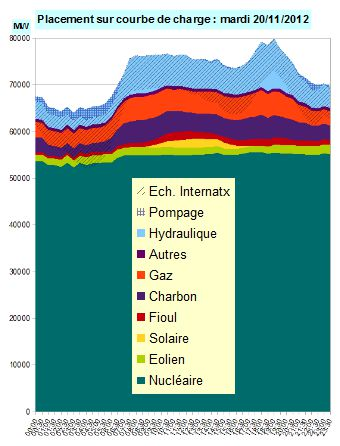
\includegraphics[width=0.5\textwidth]{images/problematique/ccharge.jpg}
 \end{center}
 \caption{Placement du type d'énergie sollicitée sur la courbe de charge 
française du mardi 20 novembre 2012 (à remplacer par une plus 
belle/récente)(source RTE)}
 \label{fig:courbeCharge}
\end{figure}

Ces pics connaissent une intensification significative avec 
l'émergence de nouveaux usages de consommation dont, notamment, la mobilité 
électrique. En France, les pouvoirs publics estiment à deux millions le nombre 
de véhicules 
électriques en circulation en 2020. L'impacte de ces véhicules sur l'équilibre 
entre l'offre et la demande n'est pas négligeable. En effet, la recharge 
complète d'un véhicule électrique ayant 150 km d'autonomie est équivalente en 
terme d'appel de puissance à~:
\begin{itemize}
\item un chauffe-eau si la recharge s'effectue en 8~h (recharge normale)~;
\item un immeuble si la recharge s'effectue en 1~h (recharge accélérée)~;
\item un quartier urbain si la recharge s'effectue en 3~min (recharge rapide).
\end{itemize}



\subsection{Architecture des Smart Grids : vers des réseaux électriques 
flexibles et communicants}

Pour faire face aux mutations du contexte énergétique, les gestionnaires de 
réseaux électriques ne peuvent plus uniquement compter sur la conduite 
prévisionnelle du réseau (pas assez réactive face à l'intermittence des énergies 
renouvelable par exemple) ni sur son redimensionnement (onéreux et non optimal). 

La solution réside dans l'acquisition en temps réel d'informations utiles 
permettant une conduite automatique et flexible des réseaux électriques. 
L'automatisation passe par un déploiement massif des TIC au niveau de 
l'infrastructure électrique. Ainsi équipés, les réseaux électriques 
s'apparentent à une toile d'araignée où les mailles interagissent 
constamment via les liens de communication. Ces mailles correspondent aux 
acteurs du système 
électrique~: consommateurs, producteurs ou les deux à la fois. 
Outre l'électricité, ces acteurs produisent et consomment de l'information en 
temps réel grâce aux modules logiciels dont ils sont équipés et à divers moyens 
de 
télécommunication (tels que les réseaux mobiles ou le CPL). Cet circulation 
permanente et instantanée de information entre les équipements préserve la 
stabilité du système électrique tout en augmentant son efficacité énergétique. 

Pour illustrer les possibilités offertes par les TIC, prenons l'exemple du pic 
de consommation de la fin de journée d'un jour en semaine. Grâce aux TIC, il 
devient possible d'agir sur la demande plutôt que sur l'offre. Via des compteurs 
intelligents installés chez les clients, les point de contrôle distants et 
moyennant des incitations tarifaires, des demandes d'effacement sont adressées 
aux consommateurs comme la coupure du chauffage pendant 15~min à 30~min d'un 
foyer ou d'un bureau 
bien isolé. Sans incidence sur le confort des consommateurs, ces demandes 
d'effacement aident à lisser la courbe de charge aux heures de pointe tout en
évitant de mobiliser des centrales de production coû	. 

Nés de la convergence des réseaux électriques et des TIC, les Smart Grids se 
composent de trois couches que nous retrouvons dans la figure 
\ref{fig:archismartgrids} :
\begin{enumerate}
\item Le premier niveau correspond aux infrastructures et équipements 
électriques acheminant l'électricité tels que les lignes et les 
transformateurs~; 
\item Le second niveau correspond à l'infrastructure de communication composée 
de différentes technologies de télécommunication comme la fibre optique, le 
courant porteur en ligne, ou encore la 3G~. 
\item Le troisième niveau correspond aux applications informatiques qui 
incarnent «~l'intelligence~» du réseau.  En utilisant des informations délivrées 
en temps réel, ces applications calculent des consignes à envoyer aux 
équipements concernés et automatisent ainsi la conduite du système électrique. 
Cette intelligence est centralisée au niveau des centres de conduites du réseau 
ou distribuées sur les équipements électriques.
\end{enumerate}


\begin{figure}[!htbp]
 \begin{center}
  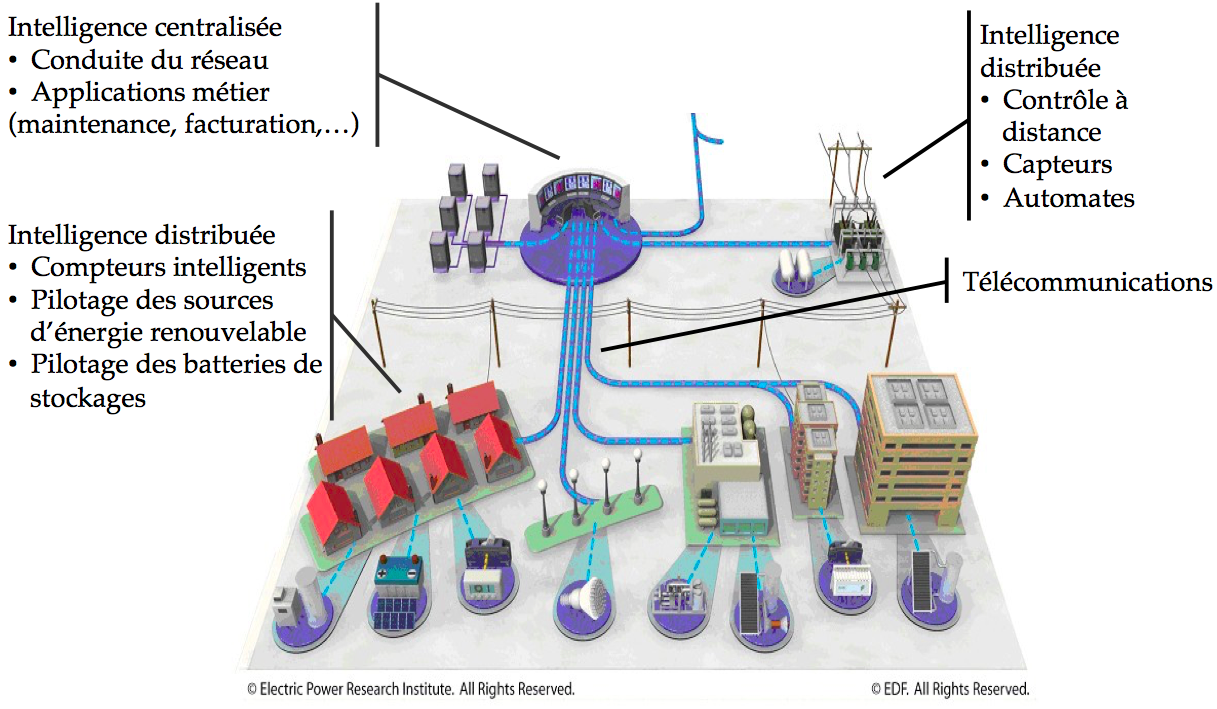
\includegraphics[width=1\textwidth]{images/problematique/archiSmartgrids.png}
 \end{center}
 \caption{Architecture des Smart Grids \protect\cite{favre2006ingenierie}}
 \label{fig:archismartgrids}
\end{figure}


%En effet, la libéralisation du marché de l'électricité exige que le 
%consommateur ait une connaissance en temps réel de l'évolution tarifaire 
horaire 
%de l'électricité et qu'il puisse même choisir d'injecter sa propre propre 
%production d'énergie sur le réseau.

\section{Problématique industrielle : la nécessaire évolution des Systèmes 
d'Information pour mettre en œuvre une stratégie orientée Smart Grids}

%Un Smart Grid est un réseau électrique intelligent permettant d'optimiser la 
%production, la distribution et la consommation d'électricité grâce à 
%l'introduction des Technologies de l'Information et de la Communication (TIC) 
%sur le réseau électrique \footnote{www.smartgrids-cre.fr}.

En traitant les données récoltées en temps réel par les capteurs installés sur 
les équipements électriques et chez les consommateurs, les SI calculent des 
consignes destinées à des organes 
télécommandés permettant ainsi de piloter les réseaux électriques à distance. 
Cette automatisation permet de mieux gérer les réseaux en les adaptant 
rapidement aux contraintes induites par l'intégration des énergies renouvelables 
et des nouveaux usages \cite{cre}. Les SI sont donc au cœur des enjeux Smart Grids.  

L'implémentation des Smart Grids va ainsi de pair avec la mise à niveau des SI 
des gestionnaires du réseau électrique. En effet, ces SI doivent pleinement 
intégrer les évolutions qu'induisent les Smart Grids aussi bien au niveau des 
processus métier de l'entreprise, des acteurs impliqués, des informations 
échangées que des applications informatiques et des infrastructures techniques 
sous-jacentes. Parmi ces évolutions nous citons~:
\begin{itemize}
\item les nouveaux flux d'information provenant du réseau électrique~;
\item l'entrée en jeu de nouveaux acteurs tels que les producteurs décentralisés 
(éolien, photovoltaïque)~;
\item les nouveaux équipements communicants comme le compteur Linky (ERDF 
annonce le déploiement de 30 millions de compteurs d'ici 
2020\footnote{www.erdf.fr/Linky})~;
\item les nouvelles réglementations et directives européennes (dans le cas des 
gestionnaires de réseaux européens)~;
\item les nouveaux usages comme les véhicules électriques ou encore les maisons 
connectées.
\end{itemize}

Outre leurs SI, les gestionnaires de réseaux électriques doivent faire évoluer 
leurs stratégies de développement en envisageant de nouveaux modèles métier et 
de nouveaux partenaires, tout en tenant compte de l'émergence des nouvelles 
technologies et des exigences du législateur. Une étude américaine, menée par 
IBM, CISCO, EPRI et South Carolina Edison, fait état de cinq thèmes stratégiques 
clés pour l'implémentation des Smart Grids~:
\begin{itemize}
\item \textbf{permettre au consommateur de contrôler sa consommation d'énergie} 
et de réduire son emprunte carbone en utilisant des équipements intelligents et 
des véhicules électriques et en produisant de l'énergie renouvelable à 
domicile~;
\item \textbf{améliorer la sécurité et la productivité des employés} en mettant 
à leur disposition des outils performants pour le contrôle à distance des 
équipements de protection et des applications mobiles par exemple~;
\item \textbf{intégrer des sources d'énergie renouvelables} distribuées sur le 
réseau en assurant la protection des équipements électriques, le stockage de 
l'énergie et la stabilité du réseau~;
\item \textbf{améliorer l'efficience et la résilience du réseau} à travers les 
systèmes de mesure en temps réel, l'analyse et le contrôle à distance~;
\item \textbf{fournir les informations et la connectivité nécessaires} à travers 
le développement d'une infrastructure TIC permettant de répondre aux besoins 
d'informatisation nécessaires à la réalisation des points précédents. Ce dernier thème est une condition sinequanone de la réalisation les quatre précédents.
\end{itemize}

Compte tenu de ces différents thèmes clés, les gestionnaires de réseaux envisagent différentes stratégies impliquant l'adoption de technologies Smart Grids. 
La mise en œuvre effective de ces stratégies demande l'automatisation des 
actions sur le réseau et du traitement des données induisant et entrainent donc le 
déploiement de nouveaux SI. Afin d'appréhender ces paradigmes naissants, plusieurs scénarios métier sont élaborés mais il est indispensable de les éprouver et de les
valider avant d'envisager leur implémentation finale.

Plusieurs démonstrateurs physiques ont été déployés sur le terrain 
\footnote{www.erdf.fr/Carte\_demonstrateurs\_Smart\_Grids}. Ces projets pilotes 
permettent de mener des expérimentations en conditions réelles pour tester des 
fonctions et des services comme par exemple le démonstrateur InfiniDrive 
\footnote{avem.fr/actualite-erdf-et-le-groupe-la-poste-lancent-le-projet-infini-drive-a-nice-3450.html} 
pour le pilotage des infrastructures de recharge de véhicules électriques ou le 
démonstrateur Venteea \footnote{www.venteea.fr} pour l'intégration de forte 
capacité éolienne dans un réseau rural. Cependant, les démonstrateurs 
nécessitent que le gestionnaire de réseau de distribution recrute des clients 
industriels et/ou domestiques qui acceptent d'avoir du matériel à tester chez 
eux. De plus, leur exploitation reste limitée par les réglementations en cours. 
Enfin, leur mise en place se révèle souvent longue et coûteuse. 

En plus de ces démonstrateurs, des réseaux de distribution d'expérimentation 
grandeur nature comme Concept Grid \footnote{chercheurs.edf.com}, implanté à EDF 
Lab, permettent de tester les nouveaux équipements avant leur installation sur 
les réseaux du distributeur ERDF\footnote{Électricité Réseau Distribution 
France}. Ces réseaux ont l'avantage de permettre la conduite de stress tests en 
conditions perturbées, impossibles à réaliser dans le cadre de démonstrateurs, 
ceux-ci impliquant de vrais clients. Cependant, la taille réduite de ces réseaux 
reste limitante.

Pour palier toutes ces limitations, une troisième voie est la simulation. Cette 
simulation intègre les trois couches composant les Smart Grids~: 
l'infrastructure électrique (transformateurs, lignes, charges, sources), 
l'infrastructure de télécommunication (réseaux mobiles, CPL \footnote{Courant 
Porteur en Ligne}) et enfin les SI qui les pilotent. Des simulateurs spécialisés 
dans la simulation de réseaux électriques (EMTP-RV, Dymola, PowerFactory, 
Eurostag, etc.) ainsi que des simulateurs de réseaux de télécommunication 
(OPNET, NS-3, OMNeT ++, etc.) ont déjà validé l'apport de la simulation dans 
leurs domaines respectifs. Toutefois, les SI sont souvent relégués à de simples 
modèles de calcul de consignes souvent développés en Matlab ou en C++ 
\cite{palensky2014simulating}. 

Dans ce contexte, la problématique industrielle dans laquelle  s'inscrivent nos 
travaux de recherche est donc la suivante~: 

\textbf{Comment valider une stratégie de développement orientée Smart Grids à 
travers la simulation de sa déclinaison au niveau du SI du gestionnaire du 
réseau électrique~?}

 
\section{Problématique de recherche}

Les technologies Smart Grids sont l'illustration du défi que représente 
l'évolution des TIC et l'intégration des énergies renouvelables pour les gestionnaires de réseaux 
électriques. Jeremy Rifkin évoque même «~une troisième révolution 
industrielle, fondée sur le couplage des technologies de l’Internet et des 
énergies nouvelles~» \cite{rifkin2012troisieme}. 

Mais à l'ère numérique, l'adaptation au changement rejoint les préoccupations de 
toute entreprise s'appuyant sur les TIC pour mener ses 
activités. Le très haut niveau de concurrence que connait le secteur des 
technologies de l'information stimule l'innovation. Or ces technologies sont de plus en plus le moteur qui fait progresser les  métier de 
l'entreprise. Être capables de s'adapter continuellement à l'évolution rapide et 
constante des TIC représente donc un véritable 
challenge pour les entreprise d'aujourd'hui. 

Or pour mener tout changement, il est primordiale de commencer par une 
description représentative de «~l'objet~» à changer, qu'il s'agisse d'une nouvelle 
version d'un avion, d'une voiture, d'un ordinateur ou encore d'une entreprise \cite{zachman1997enterprise}.

Cette description représentative revient à concevoir l'architecture de l'objet 
en question. L'architecture est une activité centrale dans plusieurs 
disciplines, allant de l'architecture du bâtiment à l'architecture logicielle, 
en ce qu'elle est un outil indispensable à la construction d'artefacts 
respectant les qualités attendues de l'objet final. En précurseur, Zachman \cite{zachman1997enterprise} recommande d'appliquer les principes d'architecture à l'entreprise pour faire face aux impératifs de changements dictés par l'innovation technologique.

Les SI étant les premiers concernés par l'évolution des technologies de 
l'information, nos travaux se sont d'abord portés sur l'évaluation de leur impact 
sur les SI de l'entreprise. De ce fait, nous nous sommes d'abord appliqués à 
décrire l'architecture de ces SI (article inforsid). 

Les changements apportés par ces technologies impliquent cependant non seulement 
les SI mais l'entreprise dans son ensemble~: de sa stratégie à ses partenaires, 
en passant par ses objectifs, ses clients et ses processus métier. Par exemple, 
l'utilisation des véhicules électriques fait \textbf{évoluer le SI} du gestionnaire du réseau électrique qui doit mettre en place de nouvelles applications capables de 
bien gérer leur recharge. Mais il doit aussi faire 
\textbf{évoluer son modèle} métier en mettant à disposition de nouveaux contrats 
client favorisant la recharge hors de la période des pics de charge par exemple 
ou encore \textbf{créer de nouveaux partenariats} avec les constructeurs 
automobiles comme dans le cas de EDF et Renault-Nissan qui collaborent sur un 
système de recharge pour véhicule électrique permettant la transmission de 
données entre les bornes de recharge et les véhicules électriques.

Évaluer l'adoption de nouvelles technologies de l'information oblige à prendre 
en compte l'entreprise dans son ensemble afin de garantir une cohérence entre 
la stratégie d'évolution adoptée et les SI qui implémentent cette stratégie. 
C'est pour cette raison que nous adoptons l'architecture d'entreprise pour 
évaluer l'impact des technologies Smart Grids sur les gestionnaires des réseaux 
électriques car l'alignement entre la stratégie métier et le SI est au cœur de 
l'architecture d'entreprise \cite{zachman1997enterprise}. Il est en effet indispensable de concevoir une 
architecture cible pour avoir  «~une vision générale de comment une entreprise 
va mettre en œuvre sa stratégie~» \cite{ross2006enterprise}.

De plus, l'architecture d'entreprise en offrant une vision globale et transverse 
de l'entreprise \cite{zachman1987framework}. Dans le cas des Smart Grids par 
exemple, elle permet d'aligner efficacement les intérêts des acteurs impliqués 
dans l'implémentation des Smart Grids tels que les experts métier, les 
conseillers stratégiques, les experts environnementaux ou encore les experts en 
normalisation.

L'exécution effective d'une stratégie est cependant confrontée à des barrières 
de communication au sein de l'entreprise \cite{vcater2010factors}. Le recours à 
l'architecture d'entreprise est d'autant plus justifié qu'elle représente un 
outil pour la transmission des objectifs stratégiques à tous les niveaux 
hiérarchiques de l'organisation en question \cite{kappelman2008enterprise}. 

En conséquence, nous souhaitons mettre à profit les principes d'architecture d'entreprise pour 
évaluer l'impact de l'adoption des technologies Smart Grids sur les SI des 
gestionnaires de réseaux électriques, tout en garantissant la cohérence entre la 
stratégie adoptée et les SI qui les implémentes. 



%\cite{buckl2010conceptual}. Le recours à l'architecture d'entreprise est ainsi 
%pleinement justifié.

Les Smart Grids s'apparente à des systèmes  dynamiques et complexes 
\cite{monti_power_2010} étant donné le grande nombre de parties prenantes qui interagissent  tout en ayant des comportements autonomes et des objectifs différents. C'est le cas par exemples des producteurs d'énergie renouvelable ou des consommateurs actifs sur le réseau électriques. La déclinaison d'une stratégie orientée Smart Grid au niveau du 
SI de la compagnie engendre ainsi des systèmes dynamiques au comportements 
complexes. \cite{borshchev2004system} affirme que le seul moyen d'adresser cette 
complexité est de simuler ces systèmes. La simulation est une technique connue 
pour valider ou critiquer la conception d'un système dès les premières étapes de 
son cycle de développement. Les acteurs impliqués dans le déploiement des 
Smart Grids acquièrent, par la  simulation, une connaissance approfondie et 
directe des modèles créés pour valider ou critiquer leur choix d'implémentation.

Néanmoins, les approches d'architecture d'entreprise se focalisent le plus souvent sur 
des aspects statiques et structurels tels que les interconnexions entre les 
différentes applications métier \cite{buckl2008towards}. De plus, les modèles 
issus de ces approches sont ne sont pas exécutables et sont conçus en priorité pour la documentation et la communication entre parties prenantes \cite{kulkarni2013modelling}. Notre 
problématique de recherche se résume de ce fait dans la question suivante :

\textbf{Quels critères doivent satisfaire les modèles issus de l'architecture 
d'entreprise pour en permettre la simulation?}
     




